\documentclass[conference]{IEEEtran}
\usepackage{cite}
\usepackage{hyperref}
\usepackage{graphicx}
\usepackage{amsmath,amssymb,amsfonts,bm}
\usepackage{algorithmic}
\usepackage{textcomp}
\usepackage{xcolor}
\usepackage[caption=false,justification=centering]{subfig}
\usepackage[export]{adjustbox}

\newcommand*{\vertbar}{\rule[-1ex]{0.5pt}{1.5em}}
\newcommand*{\horzbar}{\rule[0.5ex]{1.5em}{0.5pt}}

\def\BibTeX{{\rm B\kern-.05em{\sc i\kern-.025em b}\kern-.08em
    T\kern-.1667em\lower.7ex\hbox{E}\kern-.125emX}}
\begin{document}

\title{Analysis and Modeling of InGaZnO Thin Film Transistor Common-Gate Amplifier}

\author{Reed Foster}

\maketitle

\begin{abstract}
    In this work, a InGaZnO (IGZO) thin film transistor (TFT) common-gate amplifier and a TFT small signal model are demonstrated.
    The fabricated amplifier achieves a DC gain of nearly 2 and 3dB cutoff frequency of roughly 30kHz.
    The model integrates the intrinsic parasitic capacitances of the amplifier and accurately predicts the experimentally measured frequency response when the measurement apparatus parasitics are considered.
\end{abstract}

\begin{IEEEkeywords}
    Indium Gallium Zinc Oxide, thin film transistors, high speed analog integrated circuits
\end{IEEEkeywords}

\section{Introduction}
Amorphous thin film transistors are simple to fabricate and can be constructed on flexible substrates, making them a great platform for inexpensive wearable or embedded systems.
InGaZnO (IGZO) is a popular material for thin film transistors due to its relatively high mobility and ease of fabrication\cite{Nomura}.
Monolithic integration of analog and digital systems in IGZO could provide a solution for embedded/wearable computing and sensing,
but in order to enable the design of analog circuits in a new material system,
engineers need accurate models that quantitatively predict the behavior of their circuits across all frequencies.
Typically, this modeling is done with a small signal model of the transistor which incorporates an intrinsic transistor core and parasitic capacitance and resistance.
An accurate small signal model for a single transistor amplifier would capture virtually all of the parameters needed to model the behavior of complex, multi-transistor circuits.

To benchmark the accuracy of the small signal model, a common gate amplifier is fabricated in a three mask IGZO top gate process.
The DC current-voltage characteristics of the process are measured to extract the DC small signal parameters of the amplifier core, while the small signal capacitances are estimated based on device geometry and materials.
The small signal parameters are de-embedded, following a procedure similar to \cite{Cheng}.
The model is then compared with the experimentally measured frequency response of the common-gate amplifer.

\section{Background}

\subsection{Common Gate Amplifier}

The common gate amplifier is often used in CMOS radio-frequency (RF) applications due to its real input impedance and ability to operate near its transit frequency $f_T$ \cite{Razavi}.
While there's no gate-drain overlap capacitance $C_{gd}$ in the top-gate thin film transistor process used in this work
(and thus the degradation in bandwidth typically observed in a common source amplifier due to the Miller effect would be negligible),
a common gate amplifier was chosen over the common source configuration to minimize overlap with the projects of other students.

\begin{figure}[htbp]
    \centering
    \subfloat[]{
        
\includegraphics[width=0.35\columnwidth,valign=m]{images/common_gate_canonical.png}
        \vphantom{
\includegraphics[width=0.4\columnwidth,valign=m]{images/common_gate.png}}
        \label{fig:canonical_cg}
    }
    \quad
    \subfloat[]{
        
\includegraphics[width=0.4\columnwidth,valign=m]{images/common_gate.png}
        \label{fig:cg}
    }
    \caption{Canonical common gate amplifier configuration with resistive load and common gate amplifier with active load. $V_{b1}$ and $V_{b2}$ are DC bias voltages that can be changed to alter the operating point of the amplifier.}
    \label{fig:commongate}
\end{figure}

\subsection{Thin-Film-Transistor Small Signal Model}

\begin{figure}[htbp]
    \centering
    \subfloat[IGZO thin film transistor parasitics used in small signal model.]{
        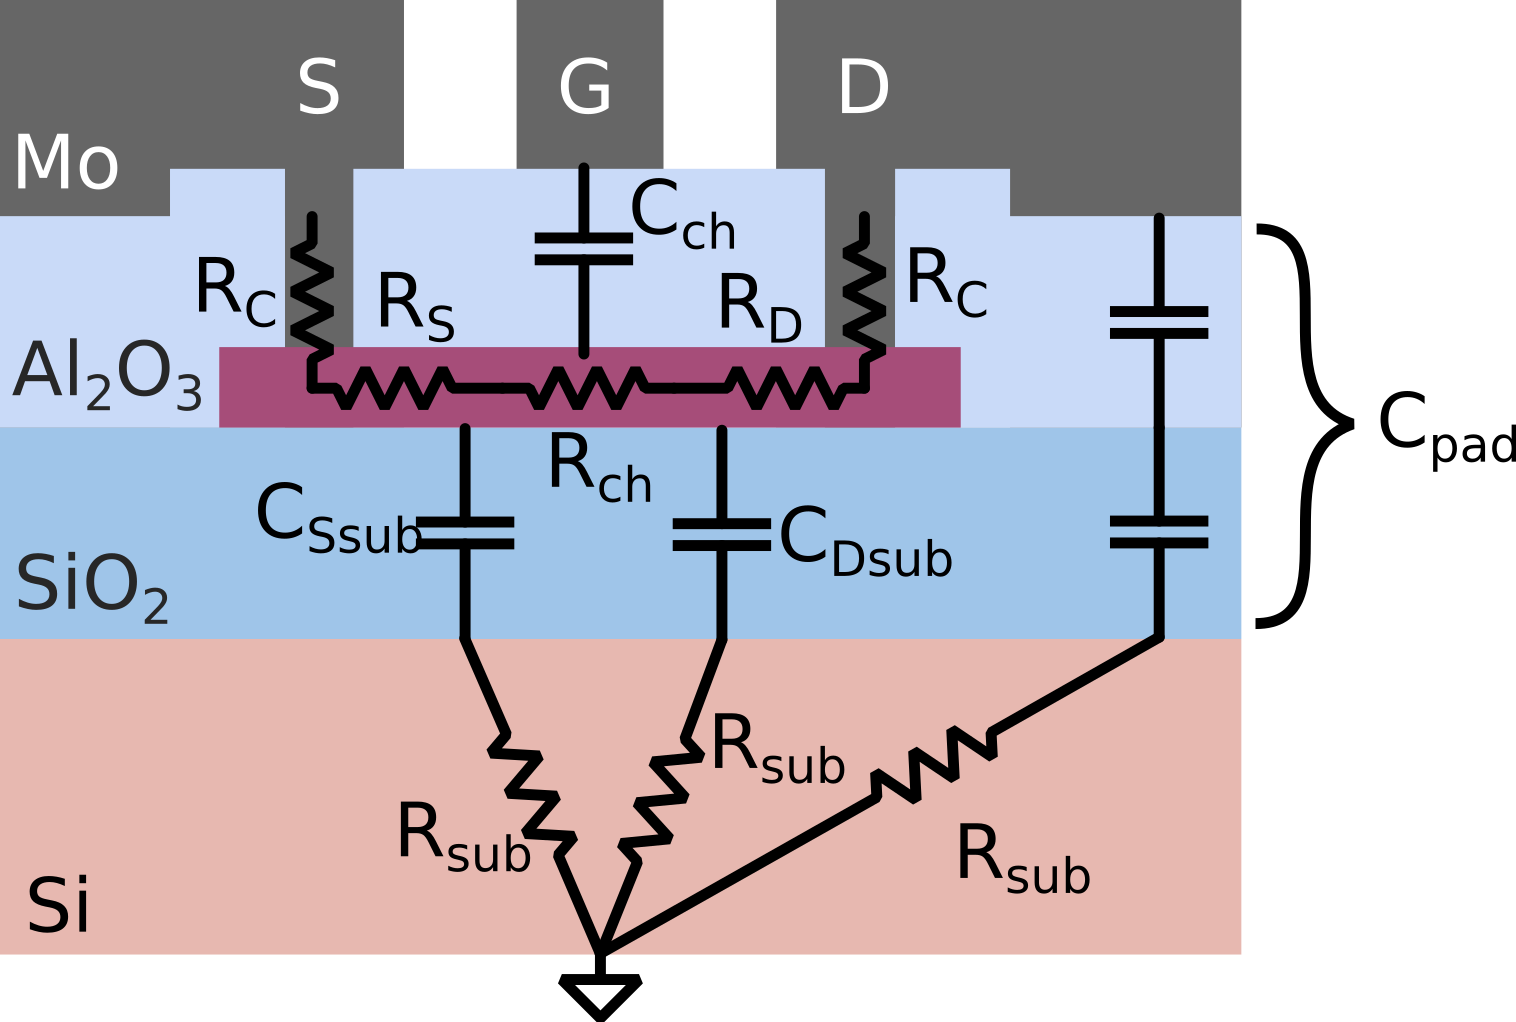
\includegraphics[width=0.52\columnwidth,valign=m]{images/capacitances.png}
        \label{fig:capacitances}
    }
    \quad
    \subfloat[Small signal model for thin film transistor]{
        
\includegraphics[width=0.35\columnwidth,valign=m]{images/tft_small_signal.png}
        \vphantom{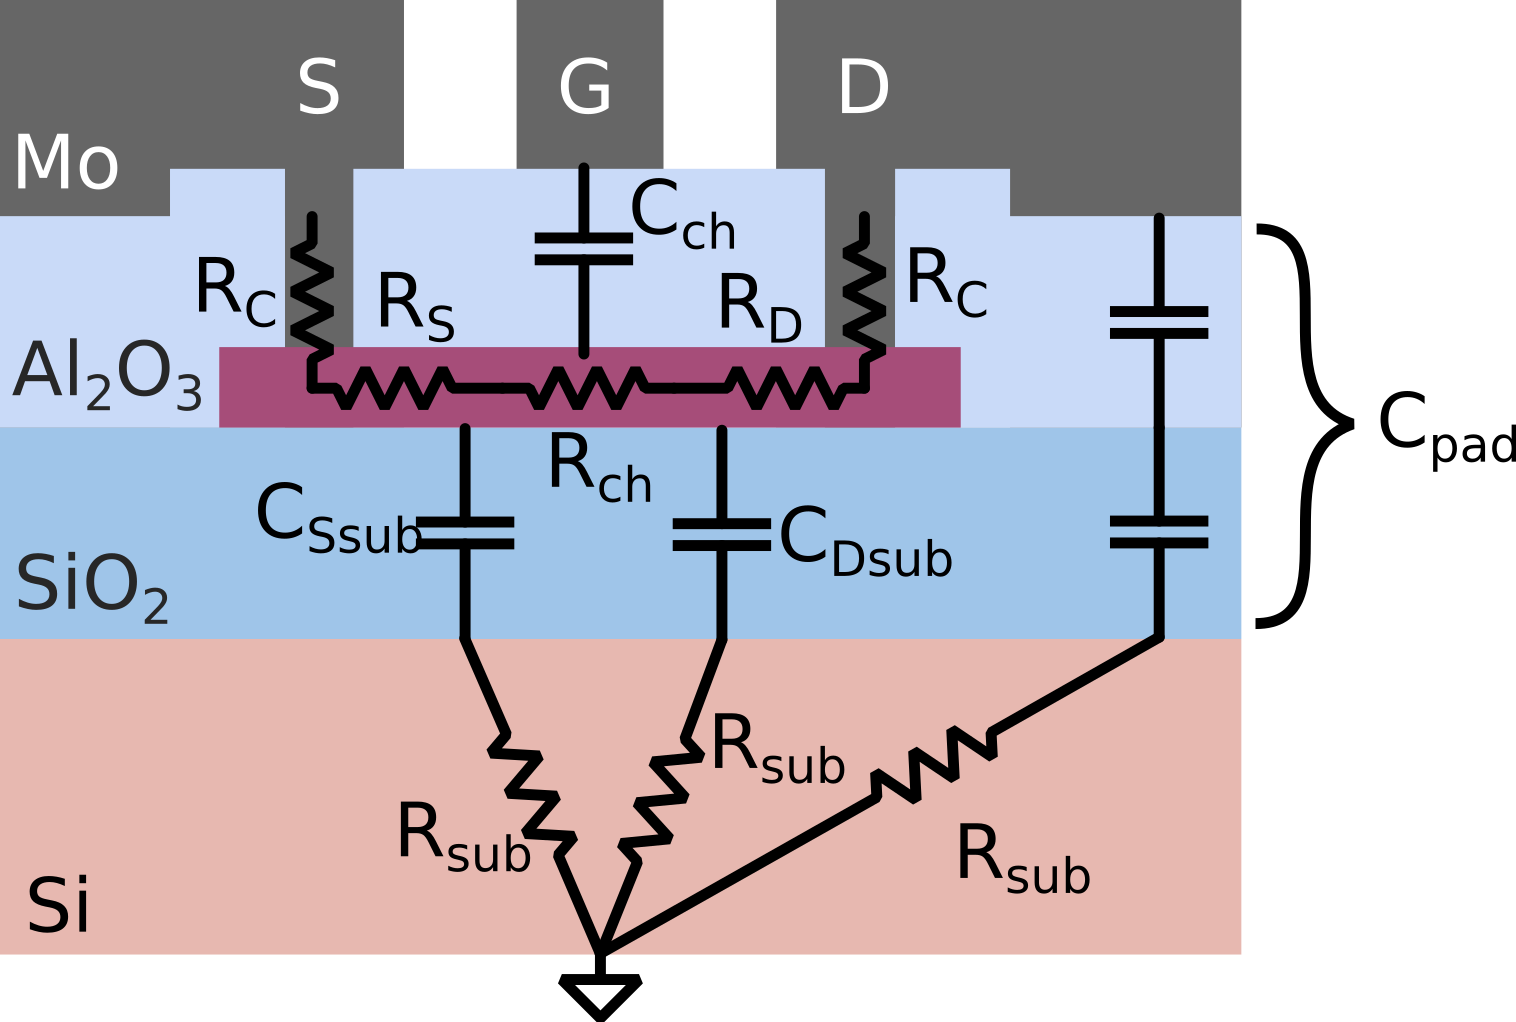
\includegraphics[width=0.52\columnwidth,valign=m]{images/capacitances.png}}
        \label{fig:tftsmallsignal}
    }
    \caption{
        IGZO thin film transistor small signal model and transistor cross section depicting origin of parasitics.
    }
    \label{fig:smallsignalmodels}
\end{figure}


Unlike in traditional MOSFETs, thin film transistors typically have large contact resistance and depending on their geometry, little to no overlap capacitance \cite{Cheng},\cite{Holland}.
In order to accurately model this effect, a new small signal model needs to be used which accounts for elevated contact resistance.
Fig. \ref{fig:capacitances} shows the various parasitic resistances and capacitances present in the top gate IGZO transistors.
The Si substrate resistance $R_{sub}$ is calculated assuming a resistivity of 100$\Omega$cm, which assumes that the substrate has been lightly doped with Boron (roughly 10$^{14}$/cm$^3$ \cite{NIST}).
The capacitances $C_{Ssub}$ and $C_{Dsub}$ are lumped capacitances to model the distributed capacitance between the bottom of the IGZO transistor channel and the substrate.
$R_C$, $R_S$, and $R_D$ model the IGZO-Mo contact resistance and IGZO source/drain extension sheet resistance (respectively).
The parasitics are combined to form the small signal model shown in Fig. \ref{fig:tftsmallsignal}.

Since the contact and sheet resistance affect the measured IV characteristics, the intrinsic transconductance $g_{mi}$ and output resistance $r_{oi}$ must be de-embedded from the measured extrinsic transconductance $g_m$ and output resistance $r_o$.
The intrinsic small signal parameters can be de-embedded by following a similar procedure to \cite{Cheng}, without making the simplifying assumption that $R_S = R_D$:

\begin{IEEEeqnarray}{rCl}
    g_m & = & \frac{\partial I_D}{\partial V_{GS}},~~ r_o = \frac{\partial V_{DS}}{\partial I_D} \\
    r_{oi} & = & r_o-R_D-(1+g_mr_o)R_S \\
    g_{mi} & = & g_m\frac{r_o}{r_{oi}}
    \label{eqn:intrinicparameters}
\end{IEEEeqnarray}

Fig. \ref{fig:smallsignal} shows a complete small signal model of the amplifier.

\begin{figure}[htbp]
    \centering
    \subfloat[]{
        
\includegraphics[width=0.55\columnwidth]{images/tft_cg_small_signal_maintransistor.png}
        \label{fig:mainsmallsignal}
    }
    \par
    \subfloat[]{
        
\includegraphics[width=0.45\columnwidth,valign=m]{images/tft_cg_small_signal_loadtransistor.png}
        \label{fig:loadsmallsignal}
    }
    \quad
    \subfloat[]{
        
\includegraphics[width=0.3\columnwidth,valign=m]{images/zsub.png}
        \label{fig:zsub}
        \vphantom{
\includegraphics[width=0.45\columnwidth,valign=m]{images/tft_cg_small_signal_loadtransistor.png}}
    }
    \caption{
        Small signal model of amplifier.
        Fig. \ref{fig:mainsmallsignal} shows the small signal model of the main amplifier.
        $Z_{Dsub1}$ and $Z_{Ssub1}$ are lumped capacitances to model the capacitance between the IGZO channel and the silicon substrate.
        $Z_{pad,sub}$ is the capacitance between the output metal pad and the silicon substrate.
        Fig. \ref{fig:loadsmallsignal} shows the small signal model for the load transistor M$_2$ input impedance ($Z_{M_2}$) as seen by the drain of the amplifier transistor M$_1$.
    }
    \label{fig:smallsignal}
\end{figure}

\section{Device Fabrication}

The common gate amplifier was fabricated with two transistors that share an IGZO mesa as shown in Fig. \ref{fig:probestation}.
Both transistors have a 5$\mu$m channel with 2$\mu$m ungated source/drain extensions.
The active transistor M$_1$ is 80$\mu$m wide and the load transistor M$_2$ is 30$\mu$m wide.
Fig. \ref{fig:fab} shows the steps of the fabrication process.
The devices were fabricated on a 6" p-type silicon wafer (Fig. \ref{fig:fab1}).
Plasma-enhanced chemical vapor deposition was used to deposit 420nm of SiO$_2$ on the wafer surface (Fig. \ref{fig:fab2}).
Then, 8nm of IGZO was RF sputtered at 100W with flowrates of 20sccm Ar and 1sccm O$_2$ at 1mtorr (Fig. \ref{fig:fab3}).
AZ3312 photoresist and AZ726 developer were used for photolithography of the transistor channel.
The exposed IGZO was etched with 1:9 HCl:H$_2$O for 10s (Fig. \ref{fig:fab4}).
30nm of Al$_2$O$_3$ was deposited with atomic layer deposition (Fig. \ref{fig:fab5}).
The oxide vias were patterned with 10um AZ10XT photoresist and AZ435 developer.
After a 7min spin-rinse with the developer, remaining AZ10XT and Al$_2$O$_3$ were etched in a bath of AZ435 for an additional 20min (Fig. \ref{fig:fab6}).
Next, 30nm of Mo was sputtered at 100W with 15sccm Ar at 2mtorr (Fig. \ref{fig:fab7}).
Finally, the Mo was patterned with 1um thick AZ3312 photoresist and AZ726 developer.
The exposed Mo was peroxide etched to form the metal contacts for the gate drain and source of the transistor (Fig. \ref{fig:fab8}).

\begin{figure}[htbp]
    \centering
    %\includegraphics[width=0.9\columnwidth]{process_steps.pdf}
    \subfloat[]{
        
\includegraphics[width=0.4\columnwidth]{images/process_1.png}
        \label{fig:fab1}
    }
    \quad
    \subfloat[]{
        
\includegraphics[width=0.4\columnwidth]{images/process_2.png}
        \label{fig:fab2}
    }
    \par
    \subfloat[]{
        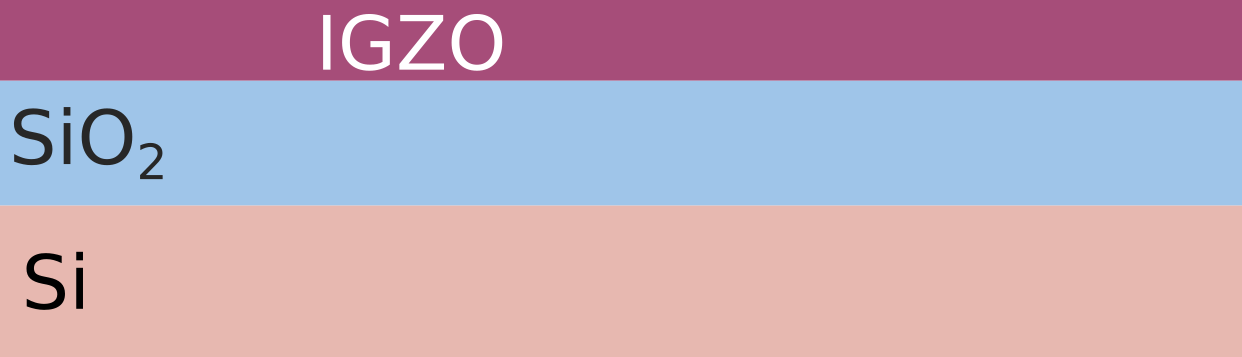
\includegraphics[width=0.4\columnwidth]{images/process_3.png}
        \label{fig:fab3}
    }
    \quad
    \subfloat[]{
        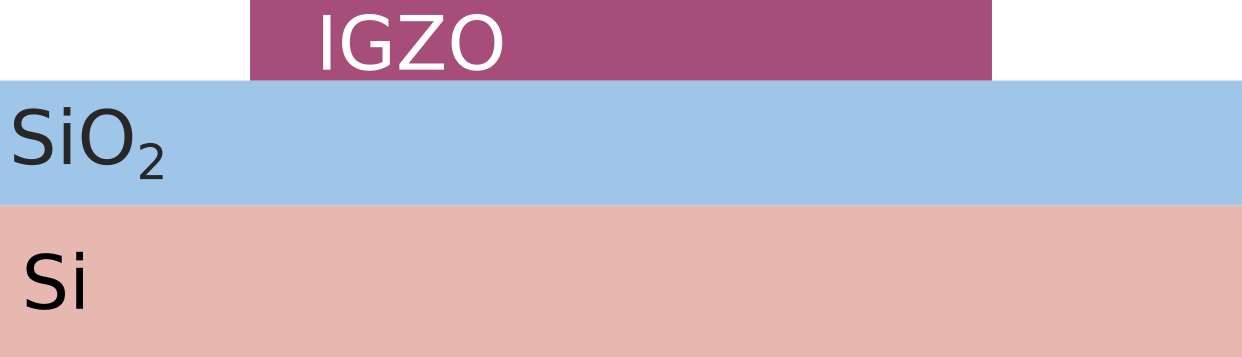
\includegraphics[width=0.4\columnwidth]{images/process_4.png}
        \label{fig:fab4}
    }
    \par
    \subfloat[]{
        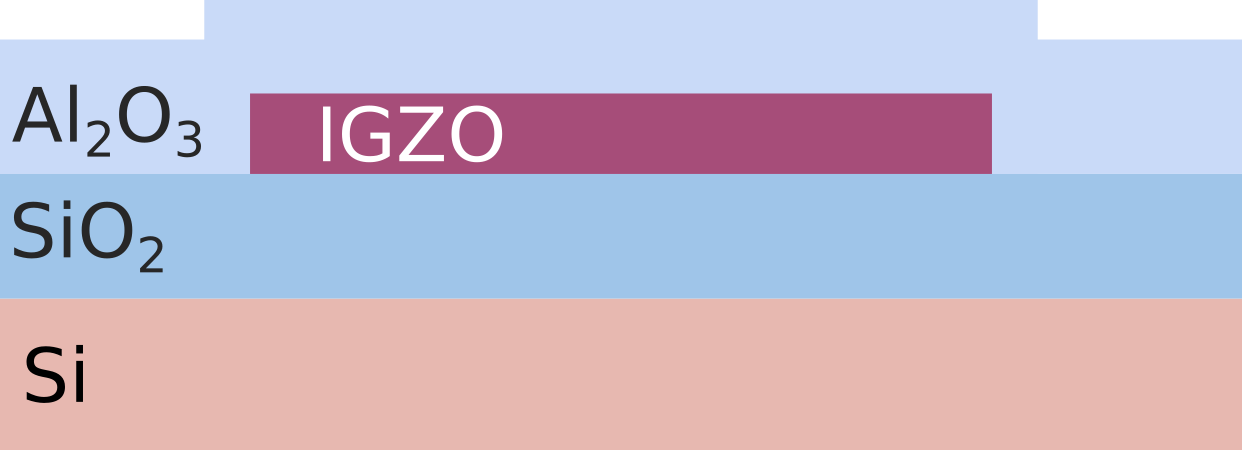
\includegraphics[width=0.4\columnwidth]{images/process_5.png}
        \label{fig:fab5}
    }
    \quad
    \subfloat[]{
        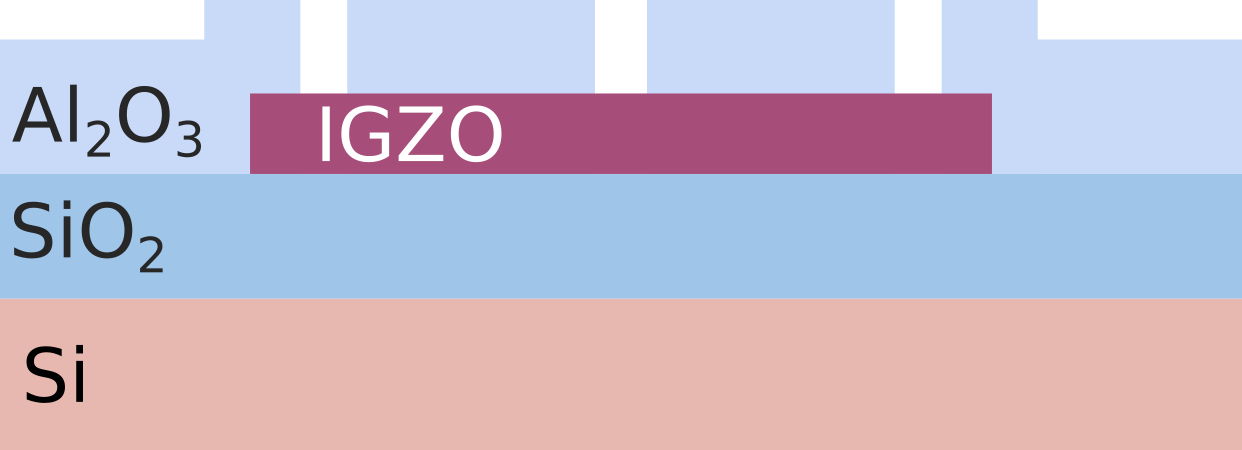
\includegraphics[width=0.4\columnwidth]{images/process_6.png}
        \label{fig:fab6}
    }
    \par
    \subfloat[]{
        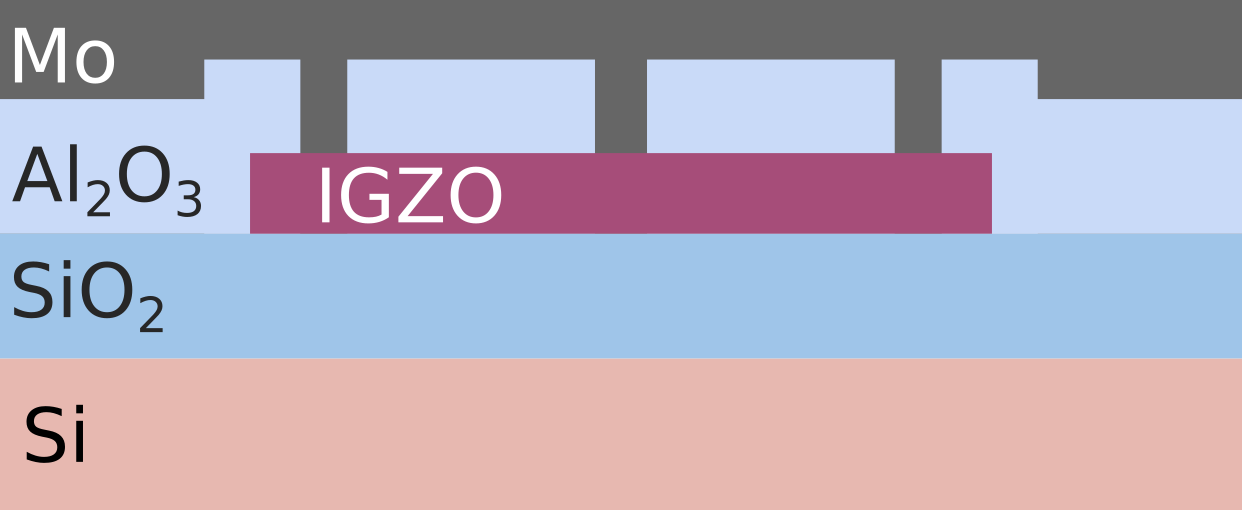
\includegraphics[width=0.4\columnwidth]{images/process_7.png}
        \label{fig:fab7}
    }
    \quad
    \subfloat[]{
        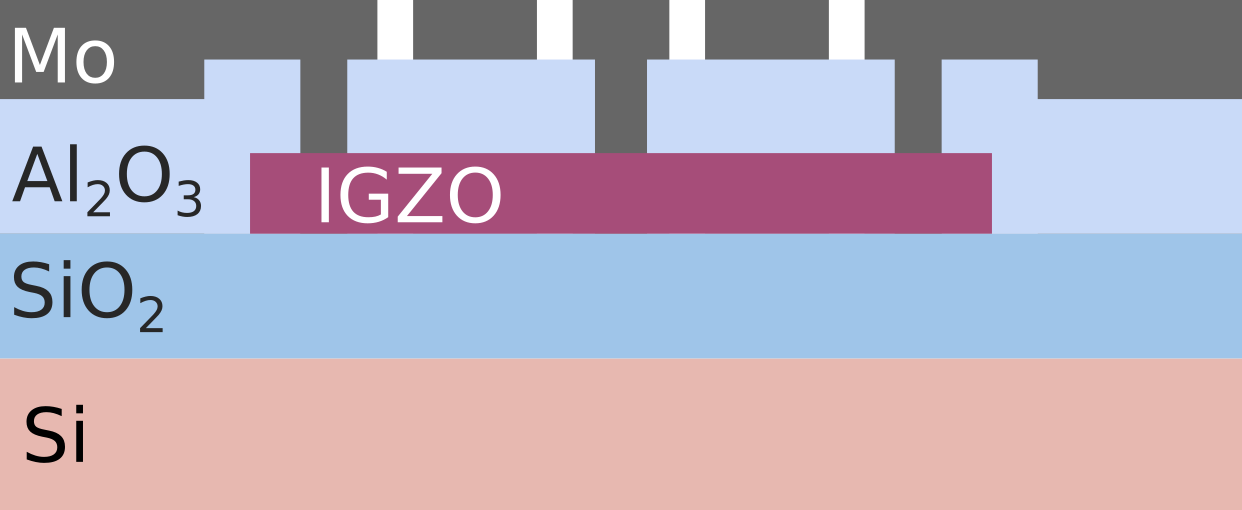
\includegraphics[width=0.4\columnwidth]{images/process_8.png}
        \label{fig:fab8}
    }
    \caption{
        Fabrication process of a pair of top-gate IGZO thin film transistors with a shared source/drain.
        Three masks are used (steps \ref{fig:fab4}, \ref{fig:fab6}, and \ref{fig:fab8}).
        This geometry can be configured as any of the single transistor amplifiers (common gate, common source, common drain).
        The common gate configuration is achieved by connecting the Mo pads (from left to right) to $v_{in}$, $V_{b1}$, $v_{out}$, $V_{b2}$, and $V_{DD}$.
    }
    \label{fig:fab}
\end{figure}

\begin{figure}[htbp]
    \centering
    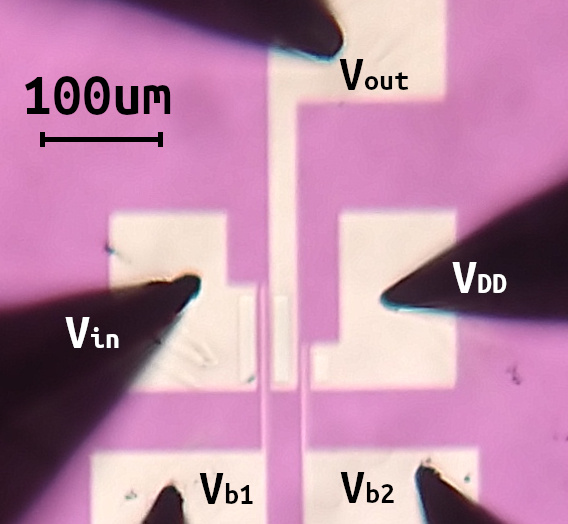
\includegraphics[width=0.6\columnwidth]{images/device_photo.jpg}
    \caption{Optical micrograph of fabricated common gate amplifier in probe station.}
    \label{fig:probestation}
\end{figure}

\section{Device Characterization and Testing}

\subsection{DC Characteristics of IGZO Process}
A Keysight B1500A semiconductor device analyzer was used to measure the DC current-voltage characteristics of the individual 80$\mu$m/5$\mu$m and 30$\mu$m/5$\mu$m transistors as shown in Fig. \ref{fig:ivmeasure}.
The semiconductor analyzer was also used to measure the contact and sheet resistance of the IGZO film using a series of two-point measurements on IGZO resistors of various dimensions.

\subsection{DC Gain and Bandwidth of Common Gate Amplifier}
The common gate amplifier is configured as shown in Fig. \ref{fig:cg} with the 80$\mu$m/5$\mu$m transistor (M$_1$) used as the amplifying transistor and the 30$\mu$m/5$\mu$m transistor (M$_2$) was used as an active load.
The differential DC gain $\Delta V_{out}/\Delta V_{in}$ was also measured with the semiconductor device analyzer to determine an appropriate bias point for optimal DC gain.

\begin{figure}[htbp]
    \centering
    \subfloat[]{
\includegraphics[width=0.33\columnwidth,valign=m]{images/common_gate_iv_measurement.png}\label{fig:ivmeasure}}
    \quad
    \subfloat[]{
\includegraphics[width=0.4\columnwidth,valign=m]{images/common_gate_freq_measurements.png}\label{fig:freqmeasure}}
    \caption{Experimental setups for measuring the IV characteristics of a single transistor (Fig. \ref{fig:ivmeasure}) and the frequency response of the common gate amplifier (Fig. \ref{fig:freqmeasure})}
    \label{fig:measurementsetup}
\end{figure}

See Fig. \ref{fig:freqmeasure} for a setup schematic for measurement of the amplifier's frequency response.
The frequency response of the common gate amplifier was measured with a Keysight DSOX2014A oscilloscope and a Keysight 33520A 80MHz function generator.
The function generator was set to produce a sinusoidal tone with 200mV$_{\text{pp}}$ output swing connected to the input terminal of the amplifier.
The oscilloscope was used to measure the function generator output as well as the output of the amplifier.
The amplitude ratio and relative phase of the input and output signals were measured for frequencies from 500Hz to 1MHz.
The DC biases $V_{b1}$, $V_{b2}$, and $V_{DD}$ were set with the source-measurement units of the semiconductor analyzer in standby mode.

\section{Results}

The sheet and contact resistances $R_S$, $R_D$, and $R_C$ used in the small signal model (Fig. \ref{fig:tftsmallsignal}) were extracted from Fig. \ref{fig:igzoresistance}.
The slope of the resistance vs. IGZO rectangle aspect ratio gives the sheet resistance in $\Omega/\square$ and the y-intercept is twice the contact resistance between the Mo and IGZO.
The bulk resistivity and contact resistance were estimated to be $\rho \approx 0.06\Omega\cdot$cm (good agreement with literature \cite{Hsu}) and $\rho_C \approx 0.022\Omega\cdot$cm$^2$.

\begin{figure}[h!]
    \centering
    \subfloat[Resistance vs. IGZO film aspect ratio]{
        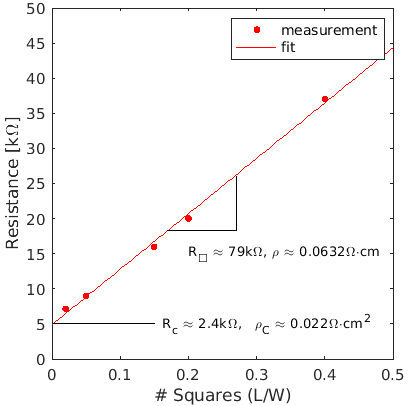
\includegraphics[width=0.5\columnwidth,valign=m]{data/resistance.png}
        \label{fig:igzoresistance}
    }
    \quad
    \subfloat[IGZO overetch]{
        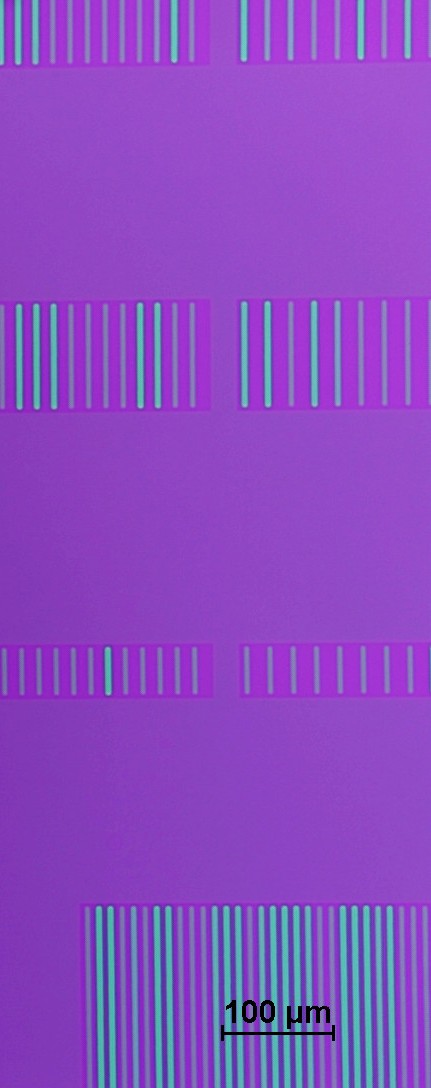
\includegraphics[width=0.2\columnwidth,valign=m]{images/overetch_t.jpg}
        \vphantom{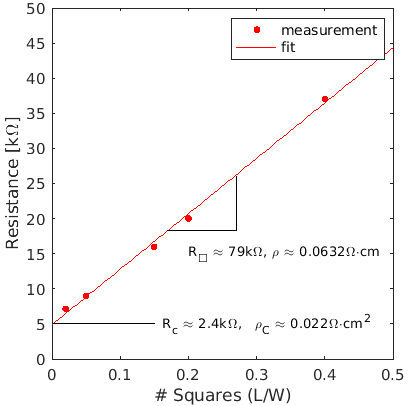
\includegraphics[width=0.5\columnwidth,valign=m]{data/resistance.png}}
        \label{fig:overetch}
    }
    \caption{Resistance of the IGZO film and properties of the IGZO-Mo interface. Fig. \ref{fig:igzoresistance} shows the results of two-point resistance measurements of 8nm thick IGZO films of varying aspect ratios. The Mo-IGZO contact area was 900$\mu$m$^2$. Fig. \ref{fig:overetch} is a contrast-enchanced optical micrograph of resistance test structures after etching of Al$_2$O$_3$ vias. Some of the IGZO has been overetched. This resulted in many non-ohmic contacts (measurements not shown).}
\end{figure}

\begin{figure}[htbp]
    \centering
    \subfloat[Transfer characteristics\\ ($W=30\mu$m, $L=5\mu$m)]{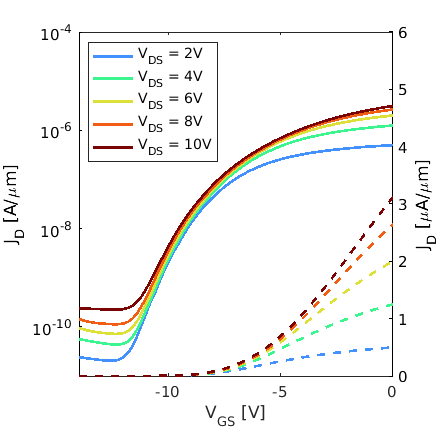
\includegraphics[width=0.48\columnwidth,trim=0px 0px 0px 25px,clip]{data/0502_30_5_transfer.png}\label{fig:30_5_transfer}}
    \quad
    \subfloat[Transfer characteristics\\ ($W=80\mu$m, $L=5\mu$m)]{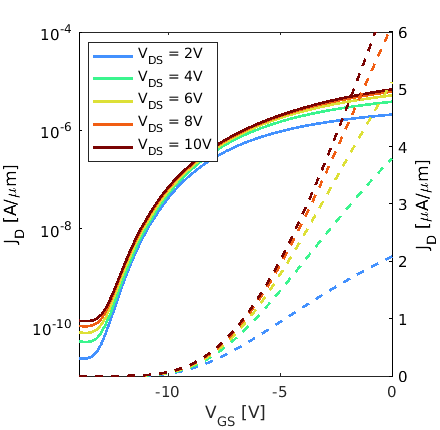
\includegraphics[width=0.48\columnwidth,trim=0px 0px 0px 25px,clip]{data/0502_80_5_transfer.png}\label{fig:80_5_transfer}}
    \par
    \subfloat[Output characteristics\\ ($W=30\mu$m, $L=5\mu$m)]{  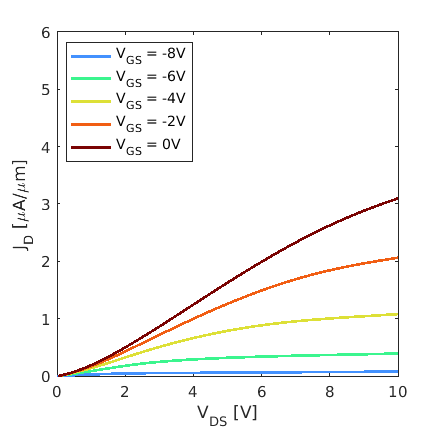
\includegraphics[width=0.45\columnwidth,trim=0px 0px 35px 30px,clip]{data/0502_30_5_output.png}\label{fig:30_5_output}}
    \quad
    \subfloat[Output characteristics\\ ($W=80\mu$m, $L=5\mu$m)]{  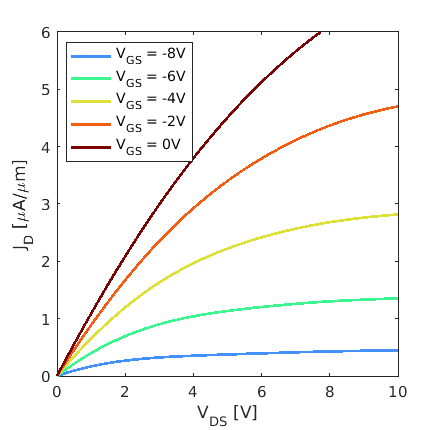
\includegraphics[width=0.45\columnwidth,trim=0px 0px 35px 30px,clip]{data/0502_80_5_output.png}\label{fig:80_5_output}}
    \caption{Transfer and output characteristics of 80$\mu$m/5$\mu$m and 30$\mu$m/5$\mu$m transistors used in the amplifier. This data was measured after weeks of testing the transistor pair in different amplifier configurations.}
    \label{fig:ivcharacteristics}
\end{figure}

Fig. \ref{fig:ivcharacteristics} shows the measured IV characteristics of the 80$\mu$m/5$\mu$m and 30$\mu$m/5$\mu$m devices.
Both demonstrate an $I_{\text{on}}/I_{\text{off}}$ ratio of about 10$^5$ and some amount of finite output resistance.
The current density (normalized to the transistor width) for the same bias point was substantially lower for the 30$\mu$m device than the 80$\mu$m device.
This is most likely due to the higher resistance of the source/drain extensions for the 30$\mu$m wide device.
The extrinsic small signal parameters $g_{m}$ and $r_{o}$ were extracted from the full set of IV data and equation \ref{eqn:intrinicparameters} was used to de-embed the intrinsic parameters $g_{mi}$ and $r_{oi}$.
The product $g_{mi}r_{oi}$ is plotted for each transistor in Fig. \ref{fig:intrinsic_gain}. $g_{mi}r_{oi}$ is the intrinsic gain of a transistor, and is the maximum possible DC voltage gain of a single transistor amplifier constructed with an ideal source and load.

%\begin{figure}[htbp]
%    \centering
%    \subfloat[Transfer characteristic in subthreshold regime\\ ($W=30\mu$m, $L=5\mu$m)]{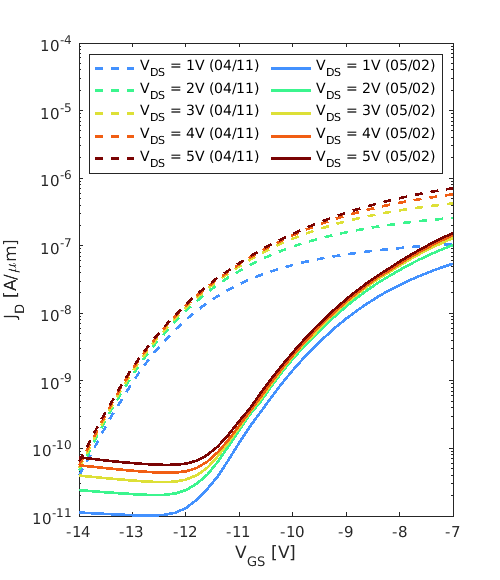
\includegraphics[width=0.4\columnwidth,trim=0px 0px 40px 40px,clip]{data/30_5_vt_degradation.png}\label{fig:30_5_vt_degradation}}
%    \quad
%    \subfloat[Transfer characteristic in subthreshold regime\\ ($W=80\mu$m, $L=5\mu$m)]{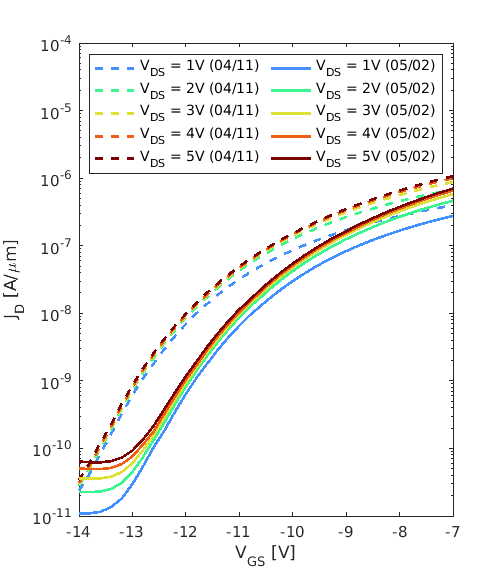
\includegraphics[width=0.4\columnwidth,trim=0px 0px 40px 40px,clip]{data/80_5_vt_degradation.png}\label{fig:80_5_vt_degradation}}
%    \caption{$V_{T}$ degradation. Initial measurements on 04/11 were taken before any other testing of the amplifier was performed. The measurements on 05/02 were taken after several weeks of testing.}
%\end{figure}

\begin{figure}[htbp]
    \centering
    \subfloat[Intrinsic gain vs. bias point\\ ($W=30\mu$m, $L=5\mu$m)]{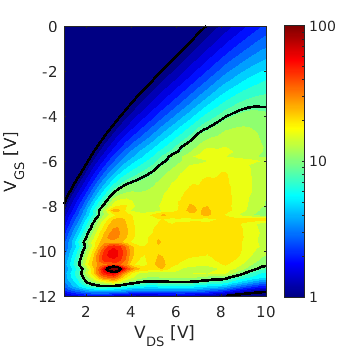
\includegraphics[width=0.48\columnwidth]{data/30_5_gmiroi.png}\label{fig:30_5_gmiroi}}
    \quad
    \subfloat[Intrinsic gain vs. bias point\\ ($W=80\mu$m, $L=5\mu$m)]{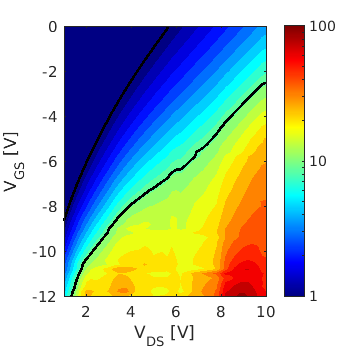
\includegraphics[width=0.48\columnwidth]{data/80_5_gmiroi.png}\label{fig:30_5_gmiroi}}
    \caption{Intrinsic gain $g_{mi}r_{oi}$ for the two transistors used in the amplifier.}
    \label{fig:intrinsic_gain}
\end{figure}

\begin{figure}[htbp]
    \centering
    \subfloat[Original small signal model]{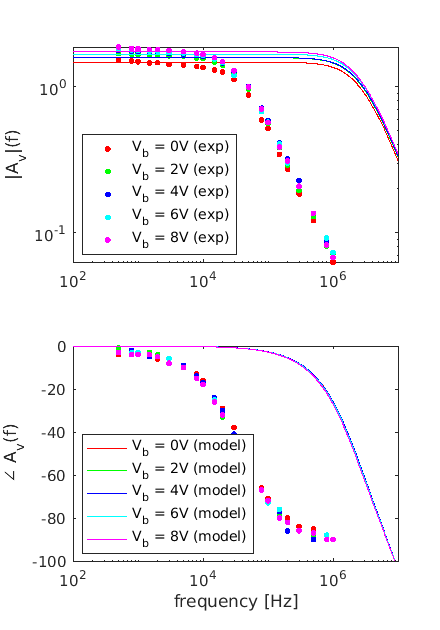
\includegraphics[width=0.48\columnwidth,trim=0px 20px 30px 46px,clip]{data/complete_small_signal_results_1xCpad.png}\label{fig:smallsignal_1xCpad}}
    \quad
    \subfloat[$C_L$ increased by 60x]{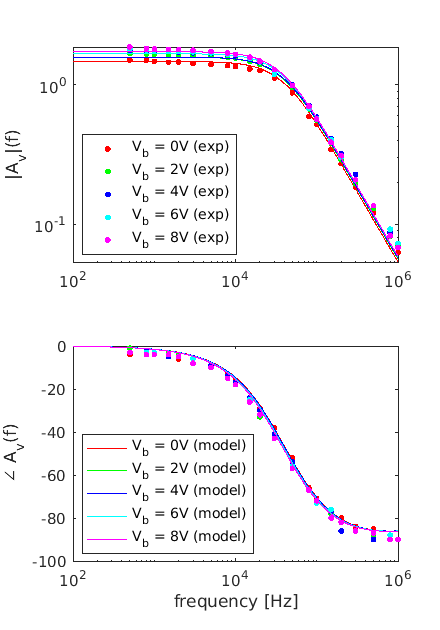
\includegraphics[width=0.48\columnwidth,trim=0px 20px 30px 46px,clip]{data/complete_small_signal_results_70xCpad.png}\label{fig:smallsignal_70xCpad}}
    \caption{Comparison of small signal model with experimental data. Points show experimental data and solid lines show the small signal model.}
    \label{fig:smallsignal_results}
\end{figure}

\section{Discussion}
%The measured bulk resistivity is roughly in agreement with literature values \cite{Lee}, \cite{Hsu}.
%As demonstrated in \cite{Park}, the resistivity of IGZO can change over orders of magnitude if treated with Ar plasma,
%so the level of agreement is reasonable.

\subsection{Small Signal Model Agreement With Experiment}

Fig. \ref{fig:smallsignal_results} shows that the small signal model correctly predicts the low frequency ($<$1kHz) gain of the amplifier quite well for the different bias points.
However, in Fig. \ref{fig:smallsignal_1xCpad}, the model overestimates the cutoff frequency of the amplifier by about 60x.
The dominant capacitance is the amplifier output node capacitance between the Mo pad and the Si substrate, and is approximately 1.7pF.
The capacitance between the IGZO channel and silicon substrate, while included in the small signal model for completeness sake, did not have a noticeable effect on the first two poles of the amplifier transfer function.
The only capacitances not accounted for in the model are the fringing capacitance between the metal contacts and the capacitance of the measurement equipment.
The fringing capacitance should be orders of magnitude lower than any of the other capacitances in the model.
However, due to the construction of the triaxial cables used with the semiconductor analyzer SMUs, they can have relatively high capacitance (as much as 90-380pF/m of cable depending on how the central guard shield is terminated in the triax-coax adapter) \cite{Tektronix}.
A load capacitance presented by the measurement equipment of just 60pF would explain the inaccuracy of the small signal model (Fig. \ref{fig:smallsignal_70xCpad}).
Therefore, the cutoff frequency of the fabricated amplifier structure should be about 1.7-1.8MHz for the same bias points (Fig. \ref{fig:smallsignal_1xCpad}).
If the large Mo pads used for measurement weren't included in the layout, i.e. in an integrated setting where the amplifier is driving some other onchip components, the cutoff frequency could be as high as 6MHz based on the other intrinsic capacitances.

In order to verify that the amplifier can function at such high frequencies, more experiments with specialized equipment, such as a network analyzer (which could calibrate out the cable capacitance), would need to be done.

\subsection{Proper Load Selection}

As configured in Fig. \ref{fig:cg}, the gain of this device as predicted by the small signal model is relatively poor.
This is because the load is effectively in a common gate configuration, and thus presents a load impedance of:
\begin{IEEEeqnarray}{rCl}
    Z_L(\omega = 0) & = & R_S + \frac{R_D + r_{oi}}{1+g_{mi}r_{oi}} = \frac{1+g_mr_oR_S+r_o}{1+g_m(R_S+r_o)} \\
    & \approx & R_S + \frac{1}{g_m} ~~ (g_mr_o \gg g_mR_S, 1)
\end{IEEEeqnarray}

If the load transistor were diode connected with the gate and source shorted together, then its input impedance would be $r_{o2}$, and the DC gain would likely be closer to the maximum gain allowed by the transistor intrinsic gain $g_{m1}(r_{o1}||r_{o2})$.
Based on the intrinsic gain $g_{mi}r_{oi}$ in Fig. \ref{fig:intrinsic_gain}, this could be as high as 10, or even 20 for a similar level of bias current.

\section{Supplemental Information and Model Code}

Measured IV curves and Matlab code for the small signal model can be found at \url{https://github.com/reed-foster/common-gate-model}.

\section*{Acknowledgment}

The author would like to thank Alon Vardy, for his help with fabrication and testing as well as many useful discussions. The author would also like to thank Karl Berggren, for lending equipment for measurement.

\begin{thebibliography}{00}
    \bibitem{Nomura} K. Nomura, et. al., ``Room-temperature fabrication of transparent flexible thin-film transistors using amorphous oxide semiconductors," Nature, vol. 432, pp. 488-492 (2004)
    %\bibitem{Kwan} T. Kwan, K. Martin, ``An Adaptive Analog Continuous-Time CMOS Biquadratic Filter," Journal of Solid-State Circuits, vol. 26, pp. 859-867 (1991)
    %\bibitem{Bahubalindruni} P. Bahubalindruni, et. al., ``High-Gain Transimpedance Amplifier for Flexible Radiation Dosimetry Using InGaZnO TFTs," Journal of the Electron Devices Society, vol. 6, pp. 760-765, (2018)
    %\bibitem{Hwang} J. Y. Hwang, M. T. Hong, E. J. Yun, B. S. Bae, ``Analog-to-digital converter with oxide thin-film transistors," Journal of Information Display, vol. 17, pp. 79-85, (2016)
    %\bibitem{Yang} T. H. Yang, et. al., ``Sparse ReRAM Engine: Joint Exploration of Activation and Weight Sparsity in Compressed Neural Networks," 2019 ACM/IEEE 46th Annual International Symposium on Computer Architecture (ISCA), pp. 236-249 (2019)
    \bibitem{Cheng} X. Cheng, S. Lee, A. Nathan ``TFT Small Signal Model and Analysis," Electron Device Letters, vol. 37, pp. 890-893, (2016)
    \bibitem{Razavi} B. Razavi, ``Fundamentals of Microelectronics," 2nd ed, Wiley, pp. 327,532-533, (2014)
    \bibitem{NIST} W. R. Thurber, R. L. Mattis, Y. M. Liu, J. J. Filliben, ``The Relationship Between Resistivity and Dopand Density for Phosphorous- and Boron-Doped Silicon," National Bureau of Standards (1981)
    \bibitem{Holland} K. Holland, et. al., ``Impact of Contact Resistance on the $f_T$ and $f_{max}$ of Graphene Versus MoS$_2$ Transistors," IEEE Trans. on Nanotechnology, vol. 16, pp. 94-106, (2017)
    %\bibitem{Lee} H. W. Lee, W. J. Cho, ``Effects of vacuum rapid thermal annealing on the electrical characteristics of amorphous indium gallium zinc oxide thin films," AIP Advances, vol. 8, 015007 (2018)
    \bibitem{Hsu} C. M. Hsu, W. C. Tzou, C. F. Yang, Y. J. Liou, ``Investigation of the High Mobility IGZO Thin Films by Using Co-Sputtering Method," Materials, vol. 8, pp. 2769-2781 (2015)
    %\bibitem{Park} J. S. Park, J. K. Jeong, Y. G. Mo, H. D. Kim, ``Improvements in the device characteristics of amorphous indium gallium zinc oxide thin-film transistors by Ar plasma treatment," Appl. Phys. Lett., vol. 90, 262106 (2007)
    %\bibitem{Muzenrieder} N. M{\"u}zenrieder, et. al., ``Flexible InGaZnO TFTs with fmax Above 300 MHz," Electron Device Letters, vol. 39, pp. 1310-1313, (2018)
    \bibitem{Tektronix} Tektronix, Appl. Note ``Making Stable Low Current Measurements with High Test Connection Capacitance Using the 4201-SMU and 4211-SMU" pp. 2-3
\end{thebibliography}


\end{document}
